\chapter{Squat Technique}

In order to ensure that the application gives appropriate feedback, it is important to discern the factors that make a squat safe and correct.

Mark Rippetoe is a well established strength coach, and has published a book entitled Starting Strength\cite{startingstrength}. This book contains detailed information regarding the biomechanics of a squat. In this project, Rippetoe's work is used as the basis for a safe squat. There are a wide range of opinions on what makes a squat safe, and no official standard has been established, however Rippetoe's work is backed by biomechanical studies and has been proved safe and effective over his years of coaching athletes. In this section the most important factors affecting the safety and optimality of a squat are discussed in turn.

\section{Depth}

One of Rippetoe's primary factors that contribute to the safety of a squat is its depth. He explains:

\begin{quote}
\emph{The squat, when performed correctly, is not only the safest leg exercise for the knees, it produces a more stable knee than any other leg exercise. The important part of the last statement is the `when performed correctly' qualifier. Correctly is deep, with hips dropping below level with the 
top of the patella.}
\end{quote}

He continues to describe the way in which a squat that does not reach sufficient depth does not stress the glutes, adductors and hamstrings, whilst it does stress the knees, resulting in an \emph{`unbalanced strain on the prepatellar area'}.

Therefore it is important that the application takes depth into account when providing feedback on the safety of a squat.

\section{Weight Distribution}

Rippetoe explains that the lifter's hips can only be used correctly with the right back angle. He elaborates that the key factor to producing the correct back angle is to ensure that the bar is directly vertical to the middle of the foot:

\begin{figure}[H]
    \centering
	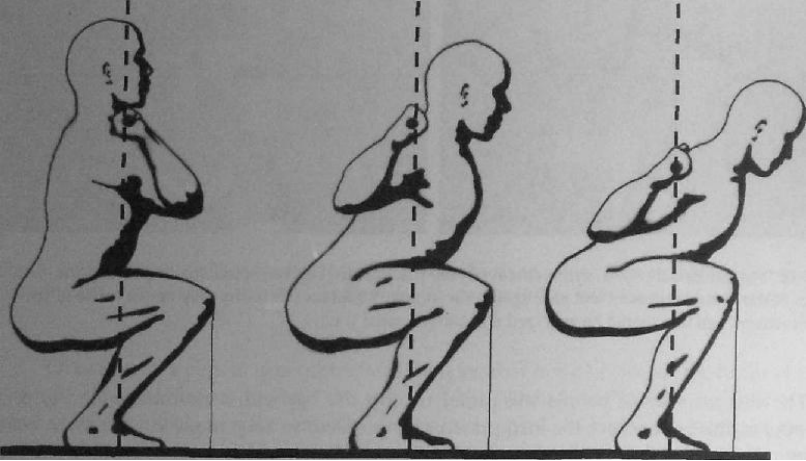
\includegraphics[height=7cm]{squat/images/rippetoe_weight_distro}
\caption{Squat weight distribution}
\label{fig:rippetoe_weight}
\end{figure}

\begin{quote}
\emph{Bar position ultimately determines back angle, as seen in this comparison of the front squat, the high-bar squat, and the low-bar squat.[\ref{fig:rippetoe_weight}] Note that the bar remains balanced over the mid-foot in each case, and this requires that the back angle accommodate the bar position.}
\end{quote}

The application should ensure that the bar is directly vertical to the foot throughout the lift.

\section{Back Angle and Knee Position}

Following on from this, there are also safety limits in the back angle and knee position. If the back angle is too close to horizontal or becomes rounded during the squat, it puts unnecessary strain on the lower back. If the back is too upright, the knees are pushed too far forward which causes strain on the patella. Rippetoe explains the detrimental effects of poor knee position:

\begin{quote}
\emph{Letting the knees travel forward at the bottom of the squat is both inefficient for posterior chain involvement and detrimental to the health of the hip flexor tendons.}
\end{quote}

He also explains the two most common problems with knee position in squats:

\begin{quote}
\emph{By far, the two most common knees errors are 1.) knees in too much and 2.) knees too far forward, either early in the descent or at the bottom.}
\end{quote}

Sadly due to the fixed position of the camera, the first error of knees buckling in towards each other cannot be addressed by the application. However this can be easily observed by the lifter when squatting in front of a mirror. The second error is straightforward to measure from a side view.

Rippetoe defines a good knee position:

\begin{quote}
\emph{Depending on your femur/tibia/trunk dimensions, your knee could be anywhere from directly above your toes to three or four inches in front of them.}
\end{quote}

The application should ensure both that the back angle is not too horizontal or vertical, and that the knees do not go too far in front of the toes.

\section{Knee and Hip Flexion}

Rippetoe also mentions the rate of relative knee and hip flexion as an important factor affecting the squat. When the angle of the knee increases at a faster rate than that of the hip in the upward stage of the squat, load is shifted to the quadriceps and away from the posterior kinetic chain (the glutes and hamstrings). This loads the spine and can open risk to injury.

This principle is shown in Starting Strength in figure~\ref{fig:rippetoe_flexion}.

\begin{figure}[H]
    \centering
	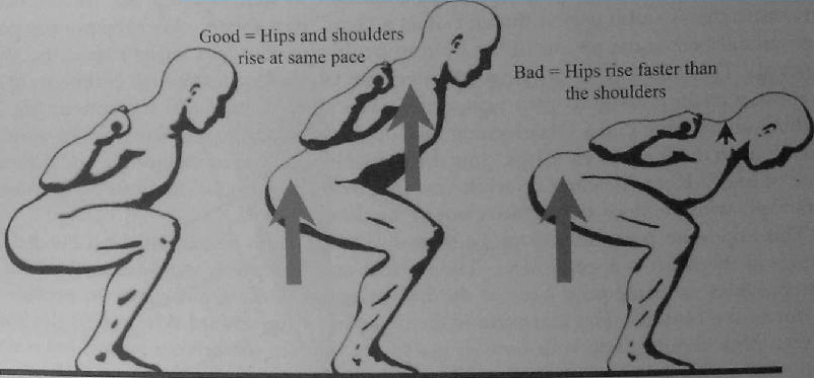
\includegraphics[height=6cm]{squat/images/rippetoe_knee_hip_flexion}
\caption{Relationship between the rate of change of the knee and hip angles}
\label{fig:rippetoe_flexion}
\end{figure}

The application should measure the rate of change of the hip and knee angles relative to one another and should penalise the lifter should the knee angle increase faster than the hip angle.

\section{Competition Rules}

The International Powerlifting Federation rules\cite{ipf} agree with Rippetoe's views on squat depth - a squat is only considered valid if the lifter descends to a point at which the hip joint is lower than the top of the knees.

The rules dictate that a squat is completed when the knees are locked and the lifter is upright. This state is known as `lockout'. The application must check that the lifter completed the full movement in order to count the squat as valid.

Another International Powerlifting Federation rule is that there should be no downward movement during the ascent stage of the squat. To have the application recognise this rule, there are two options. Either to penalise downward movement detected after starting an ascension and before locking out, or to treat any downward movement as the beginning of a new repetition. The second option allows for better segmentation of repetitions, counting squats that are not performed with the full range of motion as individual repetitions whilst penalising them appropriately for not including a lockout. The first option would only count repetitions that were fully locked out, giving a poor user experience to lifters that do not complete all of their squats successfully.